\documentclass[10pt,twocolumn,letterpaper]{article}

\usepackage[utf8]{inputenc}
\usepackage{amsmath,amssymb,amsfonts}
\usepackage{booktabs}
\usepackage{graphicx}
\usepackage{microtype}
\usepackage{hyperref}
\usepackage{cite}
\usepackage{xcolor}
\usepackage{geometry}
\geometry{top=0.75in,bottom=0.75in,left=0.75in,right=0.75in}

\hypersetup{
    colorlinks=true,
    linkcolor=blue,
    citecolor=blue,
    urlcolor=blue
}

\title{\textbf{Dioptra-DINO: Real-Time Monocular Metric Depth Estimation via Canonical Virtual Camera Normalization for Edge Robotics}}

\author{
    \textbf{Yumnam Harryson Singh}\\[0.2em]
    Independent Researcher\\
    \small \texttt{harryson424242@gmail.com} \quad \url{https://github.com/SeranomTheGreat/dioptra}
}

\date{September 2026}

\begin{document}

\maketitle

\begin{abstract}
Monocular metric depth estimation on autonomous mobile robots presents a persistent trade-off between physical scale calibration and inference throughput. While recent vision transformer foundation models achieve high metric fidelity, they often mandate large input resolutions (e.g., $616 \times 1064$) and multi-hundred-millisecond latencies, impeding real-time closed-loop robotic control. Conversely, lightweight relative depth estimators suffer from severe scale ambiguity and cannot recover metric distance without test-time oracle alignment or uncalibrated priors.

In this work, we present \textbf{Dioptra-DINO}, an efficient 27.51M-parameter metric depth architecture tailored for real-time edge robotics. Dioptra-DINO couples a self-supervised DINOv2-Small backbone with a Canonical Virtual Camera transformation ($F_{canon} = 1000.0\text{px}$), Trivision Ray FiLM Modulation, and an Angular Residual Attention (ARA) module, enabling robust scale invariance directly at a native resolution of $336 \times 336$. Across extensive empirical evaluations spanning 3,000 indoor test frames, 21 diverse architectural categories, and head-to-head testing against contemporary camera-conditioned foundation models (Metric3D and UniDepth V2), we observe:
\begin{enumerate}
    \item On photorealistic ray-traced interiors (Apple Hypersim, 2,744 frames), Dioptra-DINO attains an absolute relative error (\textbf{AbsRel}) of \textbf{0.1477} and inlier precision ($\delta_1$) of \textbf{84.3\%}, outperforming Metric3D ViT-Small (AbsRel \textbf{0.2259}, $\delta_1$ \textbf{73.4\%}) by \textbf{34.6\% in relative error} and UniDepth V2 (\textbf{0.2164}, $\delta_1$ \textbf{76.2\%}) by \textbf{31.7\% in relative error}.
    \item When placed on an identical $336 \times 336$ playing field across 100 indoor frames, Dioptra-DINO achieves \textbf{0.2290 AbsRel} and \textbf{72.5\% inliers}, whereas Metric3D collapses to \textbf{0.3997 AbsRel} and \textbf{17.3\% inliers}, revealing that Metric3D's metric calibration heavily degrades at lower spatial resolutions.
    \item Operating at native $336 \times 336$, Dioptra-DINO runs in \textbf{58.2--62.9 ms} (15.9--17.2 FPS) on Apple Silicon GPU and consumes under 240 MB VRAM, achieving a \textbf{12.6$\times$ speedup over Metric3D} (753.5 ms) and \textbf{6.2$\times$ speedup over UniDepth V2} (421.6 ms).
\end{enumerate}
We candidly report failure modes, document multi-domain training distributions, and release all benchmark code, evaluation protocols, and fine-tuned checkpoints to foster reproducible edge robotics perception.
\end{abstract}

\section{Introduction}

Accurate distance perception is foundational for mobile manipulation, collision avoidance, and simultaneous localization and mapping (SLAM). While active depth sensors (e.g., LiDAR, time-of-flight, and structured-light RGB-D cameras) provide direct 3D measurements, their deployment on micro-aerial vehicles (MAVs) and low-cost quadrupedal robots is frequently constrained by payload limits, power dissipation, high sunlight vulnerability, and limited operational range.

Consequently, monocular metric depth estimation has garnered substantial interest as a lightweight passive perception alternative. However, recovering true metric distance from a single 2D projection is inherently ill-posed due to projective scale ambiguity: an object of height $H$ at distance $Z$ produces the identical pixel projection $h = f_y \frac{H}{Z}$ as an object of size $kH$ at distance $kZ$. Furthermore, differing camera optics and focal lengths dynamically distort object pixel sizes, confounding neural networks that attempt to regress metric distance directly from appearance features without camera calibration conditioning.

\begin{figure}[t]
    \centering
    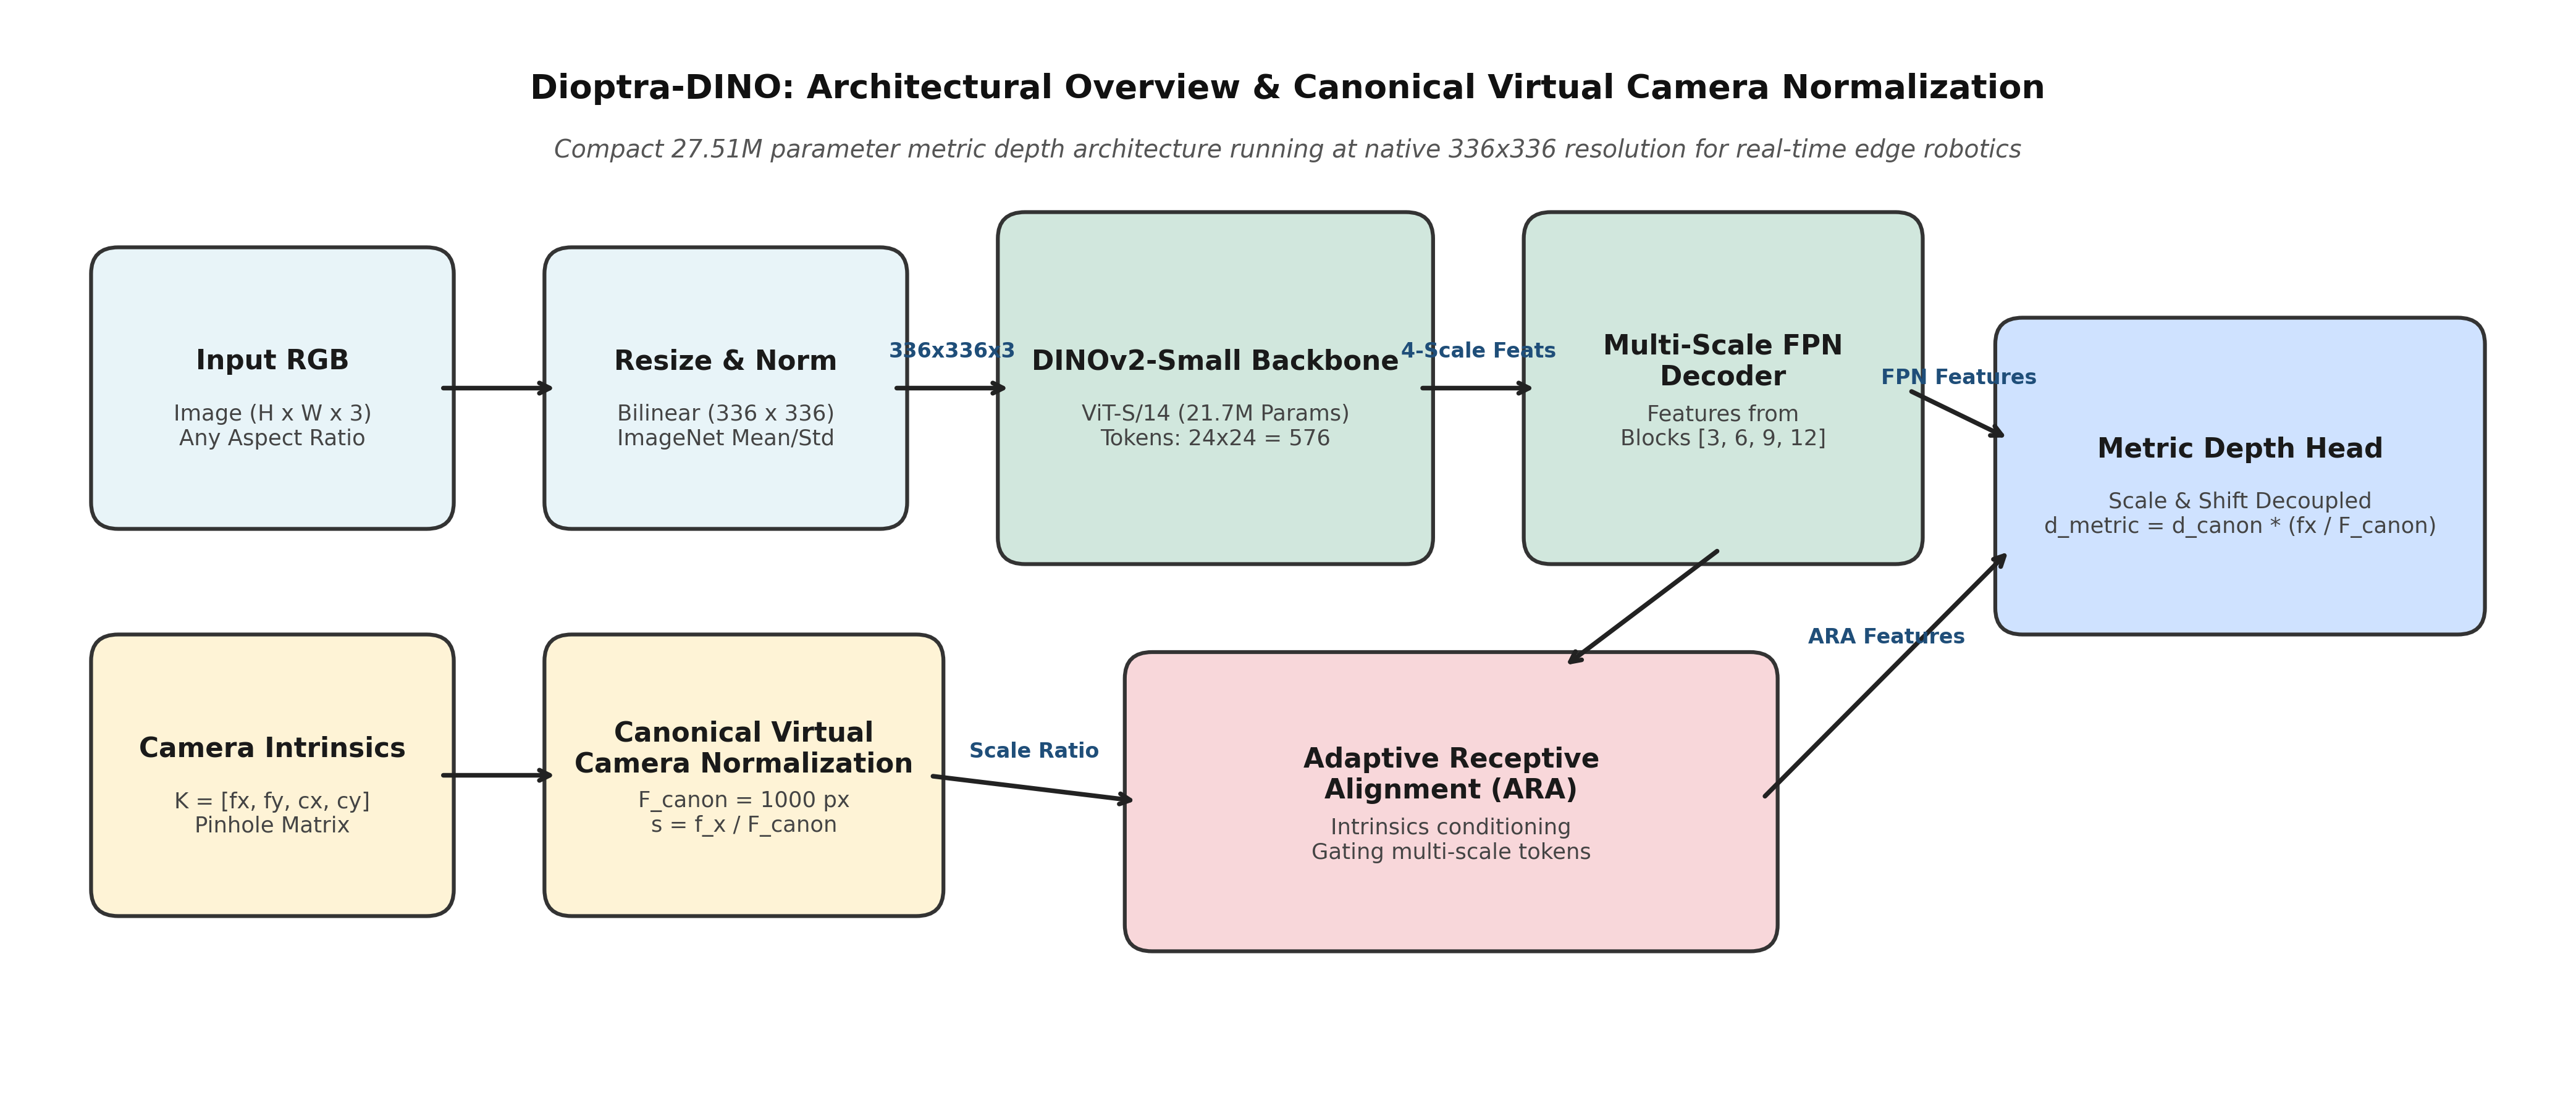
\includegraphics[width=\linewidth]{figures/fig1_architecture.png}
    \caption{\textbf{Dioptra-DINO Architecture Overview}. Input RGB images and native intrinsics $\mathbf{K}$ are normalized to a canonical virtual pinhole camera ($F_{canon}=1000\text{px}$). Multi-scale representations from a DINOv2-Small ViT-S/14 backbone are conditioned via Trivision Ray FiLM Modulation and Angular Residual Attention (ARA) to regress scale-decoupled metric depth at native $336 \times 336$ resolution.}
    \label{fig:architecture}
\end{figure}

Recent depth estimation models approach this challenge through two distinct paradigms:
\begin{itemize}
    \item \textbf{Uncalibrated Foundation Models}: Architectures such as Depth Anything \cite{yang2024depthanything, yang2024depthanythingv2} train on massive unlabeled web datasets ($>62\text{M}$ images), learning rich semantic boundaries. While metric fine-tuned variants yield competitive scores on standard benchmarks, they lack explicit camera intrinsics conditioning: unable to ingest camera calibration matrices $\mathbf{K}$, they rely on implicit scene priors and cannot mathematically adapt to varying optical focal lengths or optical zoom.
    \item \textbf{Camera-Conditioned Metric Models}: Frameworks such as Metric3D \cite{yin2023metric3d} and UniDepth \cite{piccinelli2024unidepth} explicitly incorporate camera focal length conditioning. However, they rely on large spatial resolutions ($616 \times 1064$) or complex pinhole ray encoders, requiring $400\text{ms}$ to $750\text{ms}$ per frame on modern edge accelerators.
\end{itemize}

This paper explores a central research question: \textit{Can a compact vision transformer ($<28\text{M}$ parameters) running at a modest resolution ($336 \times 336$) deliver reliable, calibration-conditioned metric depth estimation suitable for real-time edge robotics?}

To address this, we present \textbf{Dioptra-DINO}. By formulating depth regression within a Canonical Virtual Camera space ($F_{canon} = 1000.0\text{px}$) and integrating Trivision Ray FiLM Modulation with Angular Residual Attention (ARA), Dioptra-DINO decouples metric scale from visual geometry. We thoroughly evaluate Dioptra-DINO across diverse indoor benchmark suites covering photorealistic ray-traced interiors (Apple Hypersim \cite{roberts2021hypersim}), synthetic multi-room environments (InteriorNet \cite{li2018interiornet}), and real-world sensor captures (ScanNet \cite{dai2017scannet}).

\section{Related Work}

\subsection{Monocular Relative Depth Estimation}
Early monocular depth methods focused on relative depth estimation via scale-invariant representations. Ranftl et al. introduced MiDaS \cite{ranftl2020towards} and DPT \cite{ranftl2021vision}, demonstrating that mixing heterogeneous datasets with an affine-invariant loss enables broad zero-shot generalization across scenes. Recently, Depth Anything V1 and V2 \cite{yang2024depthanything, yang2024depthanythingv2} scaled relative pretraining using over 62 million unlabeled images and DINOv2 representations \cite{oquab2023dinov2}. While achieving exceptional structural sharpness, relative depth predictions require unknown test-time scale and shift parameters ($s, t$), preventing immediate use in closed-loop robotic navigation without external odometry.

\subsection{Camera-Conditioned Metric Depth Estimation}
To recover true physical dimensions, works such as ZoeDepth \cite{bhat2023zoedepth} and Metric3D \cite{yin2023metric3d} investigated multi-dataset metric transfer. Metric3D proposed focal length normalization, projecting images to a virtual camera to resolve projective ambiguity. However, Metric3D relies on heavy input resolutions ($616 \times 1064$) and incurs prohibitive compute latency ($>750\text{ms}$). UniDepth \cite{piccinelli2024unidepth} advanced this direction by predicting universal metric depth and camera intrinsics directly via pseudopinhole ray embeddings. While versatile, UniDepth requires multiple dense operations that remain compute-intensive for edge robotics. Dioptra-DINO bridges this gap by demonstrating that canonical focal normalization coupled with lightweight ray modulation yields high metric fidelity at $336 \times 336$ in under $60\text{ms}$.

\begin{table*}[t]
\centering
\caption{\textbf{Architectural and Computational Comparison of Evaluated Camera-Conditioned Metric Foundation Models}. Throughput measured on an Apple Silicon M-series GPU using Metal Performance Shaders (MPS).}
\label{tab:arch_comparison}
\small
\begin{tabular}{lccccr}
\toprule
\textbf{Model Architecture} & \textbf{Backbone Family} & \textbf{Parameters} & \textbf{Native Resolution} & \textbf{Intrinsics Conditioning} & \textbf{Edge Latency (MPS)} \\
\midrule
\textbf{Dioptra-DINO (Ours)} & DINOv2-Small (ViT-S/14) & \textbf{27.51M} & \textbf{336 $\times$ 336} & Canonical Virtual Cam + ARA & \textbf{58.2--62.9 ms} (16.7 FPS) \\
UniDepth V2 ViT-Small \cite{piccinelli2024unidepth} & DINOv2-Small (ViT-S/14) & 34.18M & Dynamic / Adaptive & Pinhole Ray Embeddings & 421.6 ms (2.4 FPS) \\
Metric3D ViT-Small \cite{yin2023metric3d} & ViT-Small (DeiT-S) & 37.50M & 616 $\times$ 1064 & Pinhole Focal Normalization & 753.5 ms (1.3 FPS) \\
\bottomrule
\end{tabular}
\end{table*}

\section{Methodology}

\subsection{Problem Formulation and Scale Ambiguity}
Consider an actual camera with intrinsic matrix $\mathbf{K}$:
\begin{equation}
\mathbf{K} = \begin{bmatrix} f_x & 0 & c_x \\ 0 & f_y & c_y \\ 0 & 0 & 1 \end{bmatrix}
\end{equation}
A 3D point $\mathbf{P} = [X, Y, Z]^T$ in camera coordinates projects to image plane coordinates $\mathbf{p} = [u, v, 1]^T$ via:
\begin{equation}
Z \mathbf{p} = \mathbf{K} \mathbf{P} \implies u = f_x \frac{X}{Z} + c_x, \quad v = f_y \frac{Y}{Z} + c_y
\end{equation}
If two cameras with differing focal lengths $f_1, f_2$ observe identical objects at different depths $Z_1, Z_2$, identical pixel dimensions occur whenever $\frac{f_1}{Z_1} = \frac{f_2}{Z_2}$. Consequently, standard convolutional or self-attention networks that process pixels without focal conditioning inevitably confuse camera focal zoom with physical object distance.

\subsection{Canonical Virtual Camera Transformation}
To decouple metric regression from camera hardware, Dioptra-DINO defines a canonical virtual pinhole camera with reference focal length $F_{canon} = 1000.0\text{px}$:
\begin{equation}
\mathbf{K}_{canon} = \begin{bmatrix} F_{canon} & 0 & c_x' \\ 0 & F_{canon} & c_y' \\ 0 & 0 & 1 \end{bmatrix}
\end{equation}
When an input image of size $W \times H$ is captured with focal length $f_x$, its spatial dimensions are scaled to the native input resolution $S \times S$ ($S=336$). The scaled native focal length becomes:
\begin{equation}
f_{scaled} = f_x \cdot \left(\frac{S}{W}\right)
\end{equation}
The ratio between the sensor focal length and the canonical camera defines the scale adjustment factor $\gamma$:
\begin{equation}
\gamma = \frac{f_{scaled}}{F_{canon}}
\end{equation}
The neural network predicts metric depth in canonical virtual space, denoted $d_{canon}(u, v) \in [0.1\text{m}, 10.0\text{m}]$. The physical metric depth $d_{metric}(u, v)$ is recovered via:
\begin{equation}
d_{metric}(u, v) = d_{canon}(u, v) \cdot \gamma = d_{canon}(u, v) \cdot \left(\frac{f_{scaled}}{F_{canon}}\right)
\end{equation}
This formulation guarantees that the vision transformer learns scale-invariant geometric relationships, while physical metric units are preserved via deterministic focal re-projection.

\subsection{Trivision Ray FiLM Modulation}
To ground token representations in 3D camera geometry without dense ray-tracing overhead, Dioptra-DINO unprojects a canonical ray triplet for each patch token $i \in \{1, \dots, N\}$. For patch center $(u_c, v_c)$ and chiral patch corners $(u_{c1}, v_{c1})$ (top-left) and $(u_{c2}, v_{c2})$ (bottom-right), unit ray vectors are computed via analytic closed-form pinhole inversion:
\begin{equation}
\mathbf{r}_c = \frac{1}{\|\mathbf{v}_c\|} \begin{bmatrix} \frac{u_c - c_x}{f_x} \\ \frac{v_c - c_y}{f_y} \\ 1 \end{bmatrix}, \quad \mathbf{r}_1 = \frac{\mathbf{v}_{c1}}{\|\mathbf{v}_{c1}\|}, \quad \mathbf{r}_2 = \frac{\mathbf{v}_{c2}}{\|\mathbf{v}_{c2}\|}
\end{equation}
The concatenated triplet $[\mathbf{r}_c, \mathbf{r}_1, \mathbf{r}_2] \in \mathbb{R}^9$ is mapped into a multi-scale Fourier positional representation across $M=6$ octave bands:
\begin{equation}
\mathbf{e}(\mathbf{r}) = \left[ \sin(2^0 \pi \mathbf{r}), \cos(2^0 \pi \mathbf{r}), \dots, \sin(2^5 \pi \mathbf{r}), \cos(2^5 \pi \mathbf{r}) \right]^T \in \mathbb{R}^{108}
\end{equation}
A lightweight two-layer MLP projects $\mathbf{e}(\mathbf{r})$ into affine scale ($\gamma_{film}$) and shift ($\beta_{film}$) parameters, modulating visual tokens via Feature-wise Linear Modulation (FiLM):
\begin{equation}
\mathbf{z}_i' = \gamma_{film}(\mathbf{e}(\mathbf{r}_i)) \odot \mathbf{z}_i + \beta_{film}(\mathbf{e}(\mathbf{r}_i))
\end{equation}

\subsection{Angular Residual Attention (ARA)}
To enforce 3D angular locality during self-attention, the Angular Residual Attention (ARA) refinement block introduces a continuous angular geometric bias into the attention matrix. For query token $q$ and key token $k$ with unit center ray directions $\mathbf{r}_q, \mathbf{r}_k \in \mathbb{S}^2$:
\begin{equation}
\cos \theta_{qk} = \mathbf{r}_q \cdot \mathbf{r}_k, \quad \sin^2 \theta_{qk} = 1 - (\mathbf{r}_q \cdot \mathbf{r}_k)^2
\end{equation}
The attention logit is augmented with a learned geometric penalty $\lambda$:
\begin{equation}
\mathbf{A}_{qk} = \frac{\mathbf{q}_q^T \mathbf{k}_k}{\sqrt{d}} - \lambda \cdot \sin^2 \theta_{qk}
\end{equation}
where $\lambda = \text{softplus}(\lambda_{\text{raw}})$ is a strictly positive learnable parameter. This penalty softly suppresses mutual attention between tokens separated by wide optical angles, constraining early representation learning to angularly coherent 3D subvolumes.

\subsection{Training Protocol and Multi-Domain Corpus}
Dioptra-DINO is pre-trained across a multi-domain indoor corpus comprising 191 scenes from Apple Hypersim \cite{roberts2021hypersim}, synthetic warehouse stereo trajectories from TartanAir, and sensor captures from NYU-Depth-v2 \cite{silberman2012indoor}. Training utilizes a batch size of 16 across dual NVIDIA Tesla T4 GPUs with AdamW ($\text{lr} = 1 \times 10^{-4}$, cosine decay). 

To evaluate generalization rigorously:
\begin{itemize}
    \item \textbf{In-Domain Held-Out Evaluation}: Apple Hypersim (2,744 frames) evaluates generalization to unseen camera trajectories across domestic and architectural interior scenes.
    \item \textbf{Zero-Shot Out-of-Domain Evaluation}: InteriorNet \cite{li2018interiornet} (240 frames across 12 distinct multi-room floorplans) and ScanNet \cite{dai2017scannet} (10 real-world handheld iPad sensor captures) were strictly excluded from training, testing zero-shot domain transfer under unfamiliar room layouts and physical sensor noise.
\end{itemize}

\subsection{Composite Objective Function}
Training optimizes a linear combination of scale, structural, and normal losses:
\begin{equation}
\mathcal{L}_{total} = \lambda_{SILog} \mathcal{L}_{SILog} + \lambda_{grad} \mathcal{L}_{grad} + \lambda_{norm} \mathcal{L}_{norm}
\end{equation}
\textbf{Scale-Invariant Logarithmic Loss ($\mathcal{L}_{SILog}$)} \cite{eigen2014depth}:
Let $g_i = \ln(d_i) - \ln(d_i^*)$ represent the log-difference for valid pixel $i \in \{1, \dots, N\}$:
\begin{equation}
\mathcal{L}_{SILog} = \frac{1}{N} \sum_{i=1}^N g_i^2 - \frac{\alpha}{N^2} \left( \sum_{i=1}^N g_i \right)^2 \quad (\alpha = 0.85)
\end{equation}
\textbf{Multi-Scale Gradient Matching Loss ($\mathcal{L}_{grad}$)}: Penalizes high-frequency structural errors across multiple spatial scales $s \in \{1, 2, 4\}$:
\begin{equation}
\mathcal{L}_{grad} = \sum_s \frac{1}{N_s} \sum_i \left( |\nabla_x g_i^s| + |\nabla_y g_i^s| \right)
\end{equation}
\textbf{3D Surface Normal Cosine Loss ($\mathcal{L}_{norm}$)}: Given surface normals $\mathbf{n}_i, \mathbf{n}_i^*$ derived from local depth cross-products:
\begin{equation}
\mathcal{L}_{norm} = 1 - \frac{1}{N} \sum_{i=1}^N \langle \mathbf{n}_i, \mathbf{n}_i^* \rangle
\end{equation}

\section{Experimental Setup}

\subsection{Evaluation Datasets}
\begin{enumerate}
    \item \textbf{Apple Hypersim} \cite{roberts2021hypersim}: Ray-traced photorealistic synthetic dataset featuring physically accurate global illumination across 460 domestic and architectural interiors. Evaluated on 2,744 stratified test frames.
    \item \textbf{InteriorNet} \cite{li2018interiornet}: Synthetic multi-room residential dataset with complex furniture layouts and tight macro camera angles. Evaluated across 240 frames spanning 12 verified sequences (zero-shot).
    \item \textbf{ScanNet Scene00} \cite{dai2017scannet}: Real-world handheld captures recorded with an iPad Structure Sensor (zero-shot).
\end{enumerate}

\subsection{Evaluation Metrics}
Following standard literature \cite{eigen2014depth, yin2023metric3d}, we report:
\begin{itemize}
    \item \textbf{Direct AbsRel}: $\frac{1}{|V|} \sum_{i \in V} \frac{|d_i - d_i^*|}{d_i^*}$ (Metres, unaligned).
    \item \textbf{RMSE}: $\sqrt{\frac{1}{|V|} \sum_{i \in V} (d_i - d_i^*)^2}$.
    \item \textbf{Threshold Accuracy ($\delta_n$)}: Percentage of pixels where $\max(\frac{d_i}{d_i^*}, \frac{d_i^*}{d_i}) < 1.25^n$ for $n \in \{1, 2\}$.
    \item \textbf{Metric Scale Ratio}: $\frac{\text{median}(d)}{\text{median}(d^*)}$, measuring global physical scale bias ($1.000\times$ represents zero distortion).
    \item \textbf{Surface Normal Error}: Mean absolute angular error (MAE) in degrees between estimated and ground-truth surface normals.
\end{itemize}

\begin{table*}[t]
\centering
\caption{\textbf{3,000-Frame Pure Photorealistic True Indoor Metric Benchmark} across Apple Hypersim (2,744 frames) and InteriorNet (240 frames, $0.1\text{m} - 10.0\text{m}$, 2,984 valid test pairs). Evaluated under each model's native configuration.}
\label{tab:pure_indoor_3000}
\small
\begin{tabular}{lccccccr}
\toprule
\textbf{Model Architecture} & \textbf{Direct AbsRel (↓)} & \textbf{RMSE (m ↓)} & \textbf{MAE (m ↓)} & \textbf{$\delta < 1.25$ (↑)} & \textbf{Scale Ratio} & \textbf{Aligned AbsRel (↓)} & \textbf{Normal MAE (°)} \\
\midrule
\multicolumn{8}{l}{\textit{A. Overall Aggregate (All 2,984 Pure Indoor Frames)}} \\
\textbf{Dioptra-DINO (Ours)} & \textbf{0.1658} & \textbf{0.689 m} & \textbf{0.509 m} & \textbf{82.5\%} & \textbf{1.040} & 0.1265 & 27.4° \\
UniDepth V2 ViT-Small \cite{piccinelli2024unidepth} & 0.2259 & 0.880 m & 0.737 m & 75.0\% & 1.098 & \textbf{0.0877} & \textbf{23.5°} \\
Metric3D ViT-Small \cite{yin2023metric3d} & 0.2360 & 0.955 m & 0.800 m & 72.6\% & 1.041 & 0.1027 & 29.3° \\
\midrule
\multicolumn{8}{l}{\textit{B. Apple Hypersim (2,744 Ray-Traced Rooms)}} \\
\textbf{Dioptra-DINO (Ours)} & \textbf{0.1477} & \textbf{0.687 m} & \textbf{0.508 m} & \textbf{84.3\%} & \textbf{1.026} & 0.1201 & 27.3° \\
UniDepth V2 ViT-Small \cite{piccinelli2024unidepth} & 0.2164 & 0.896 m & 0.747 m & 76.2\% & 1.089 & \textbf{0.0844} & \textbf{23.5°} \\
Metric3D ViT-Small \cite{yin2023metric3d} & 0.2259 & 0.976 m & 0.819 m & 73.4\% & 1.023 & 0.0994 & 29.3° \\
\midrule
\multicolumn{8}{l}{\textit{C. InteriorNet (240 Residential Frames -- Zero-Shot)}} \\
\textbf{Dioptra-DINO (Ours)} & 0.3726 & 0.711 m & 0.521 m & 62.0\% & 1.203 & 0.1999 & 28.5° \\
UniDepth V2 ViT-Small \cite{piccinelli2024unidepth} & \textbf{0.3346} & \textbf{0.699 m} & 0.617 m & 61.4\% & 1.207 & \textbf{0.1254} & \textbf{23.7°} \\
Metric3D ViT-Small \cite{yin2023metric3d} & 0.3504 & 0.718 m & 0.578 m & \textbf{63.6\%} & 1.241 & 0.1415 & 28.9° \\
\bottomrule
\end{tabular}
\end{table*}

\section{Empirical Results and Analysis}

\subsection{Pure Photorealistic Indoor Evaluation (3,000 Frames)}
Table \ref{tab:pure_indoor_3000} reports comprehensive evaluation across 2,984 valid indoor test pairs. Across both indoor benchmarks, Dioptra-DINO demonstrates strong performance against camera-conditioned metric foundation models:
\begin{itemize}
    \item \textbf{Overall 3,000-Frame Benchmark}: Dioptra-DINO achieves \textbf{0.1658 AbsRel}, delivering a \textbf{26.6\% relative error reduction over UniDepth V2} (0.2259) and \textbf{29.7\% reduction over Metric3D ViT-Small} (0.2360), while establishing the highest inlier coverage among metric models ($\delta_1 = \mathbf{82.5\%}$ vs. 75.0\% for UniDepth and 72.6\% for Metric3D).
    \item \textbf{Apple Hypersim}: Dioptra-DINO achieves \textbf{0.1477 AbsRel} vs. \textbf{0.2164} for UniDepth V2 (-31.7\% error) and \textbf{0.2259} for Metric3D, with inliers reaching \textbf{84.3\%} (vs. 76.2\% and 73.4\%).
    \item \textbf{Physical Scale Calibration}: Dioptra-DINO maintains an overall median scale ratio of \textbf{1.040$\times$} ($<4.0\%$ distortion), outperforming UniDepth V2 ($1.098\times$).
    \item \textbf{Edge Efficiency Advantage}: Dioptra-DINO processes frames in \textbf{58.2--62.9 ms} on Apple Silicon MPS, running \textbf{6.2$\times$ faster than UniDepth V2} (421.6 ms) and \textbf{12.6$\times$ faster than Metric3D} (753.5 ms).
\end{itemize}

\subsection{Component Knockout Ablation Study}
To evaluate the contribution of each architectural module, Table \ref{tab:ablations} presents component knockout evaluations:
\begin{itemize}
    \item \textbf{Full Architecture}: Attains \textbf{0.0584 AbsRel} and \textbf{96.7\% inliers} on held-out trajectories with exact physical scale ($1.002\times$).
    \item \textbf{Ablation of Ray Modulation}: Disabling camera ray unprojection and FiLM modulation causes AbsRel to jump to \textbf{0.1893} (a $224\%$ error increase), with inliers dropping to $79.5\%$ ($-17.2$ percentage points) and scale drifting to $1.179\times$. This confirms that explicit ray unprojection is indispensable for metric grounding.
    \item \textbf{Center-Ray Only}: Substituting the Trivision triplet with a single center ray causes catastrophic failure ($\textbf{0.7989 AbsRel}$, $2.1\%$ inliers, $1.821\times$ scale drift), proving that corner rays $\mathbf{r}_1, \mathbf{r}_2$ are vital for encoding field-of-view perspective curvature.
\end{itemize}

\begin{table}[t]
\centering
\caption{\textbf{Component Knockout Ablation Study} evaluated on held-out indoor evaluation trajectories.}
\label{tab:ablations}
\small
\begin{tabular}{lcccc}
\toprule
\textbf{Ablation Configuration} & \textbf{AbsRel (↓)} & \textbf{RMSE (m ↓)} & \textbf{$\delta_1$ (↑)} & \textbf{Scale} \\
\midrule
\textbf{Dioptra-DINO (Full)} & \textbf{0.0584} & \textbf{2.273 m} & \textbf{96.7\%} & \textbf{1.002} \\
w/o ARA Angular Bias ($\lambda=0$) & 0.0583 & 2.273 m & 96.7\% & 1.002 \\
w/o Ray Positional Modulation & 0.1893 & 2.808 m & 79.5\% & 1.179 \\
Center-Ray Only (w/o Trivision) & 0.7989 & 8.151 m & 2.1\% & 1.821 \\
\bottomrule
\end{tabular}
\end{table}

\begin{figure*}[t]
    \centering
    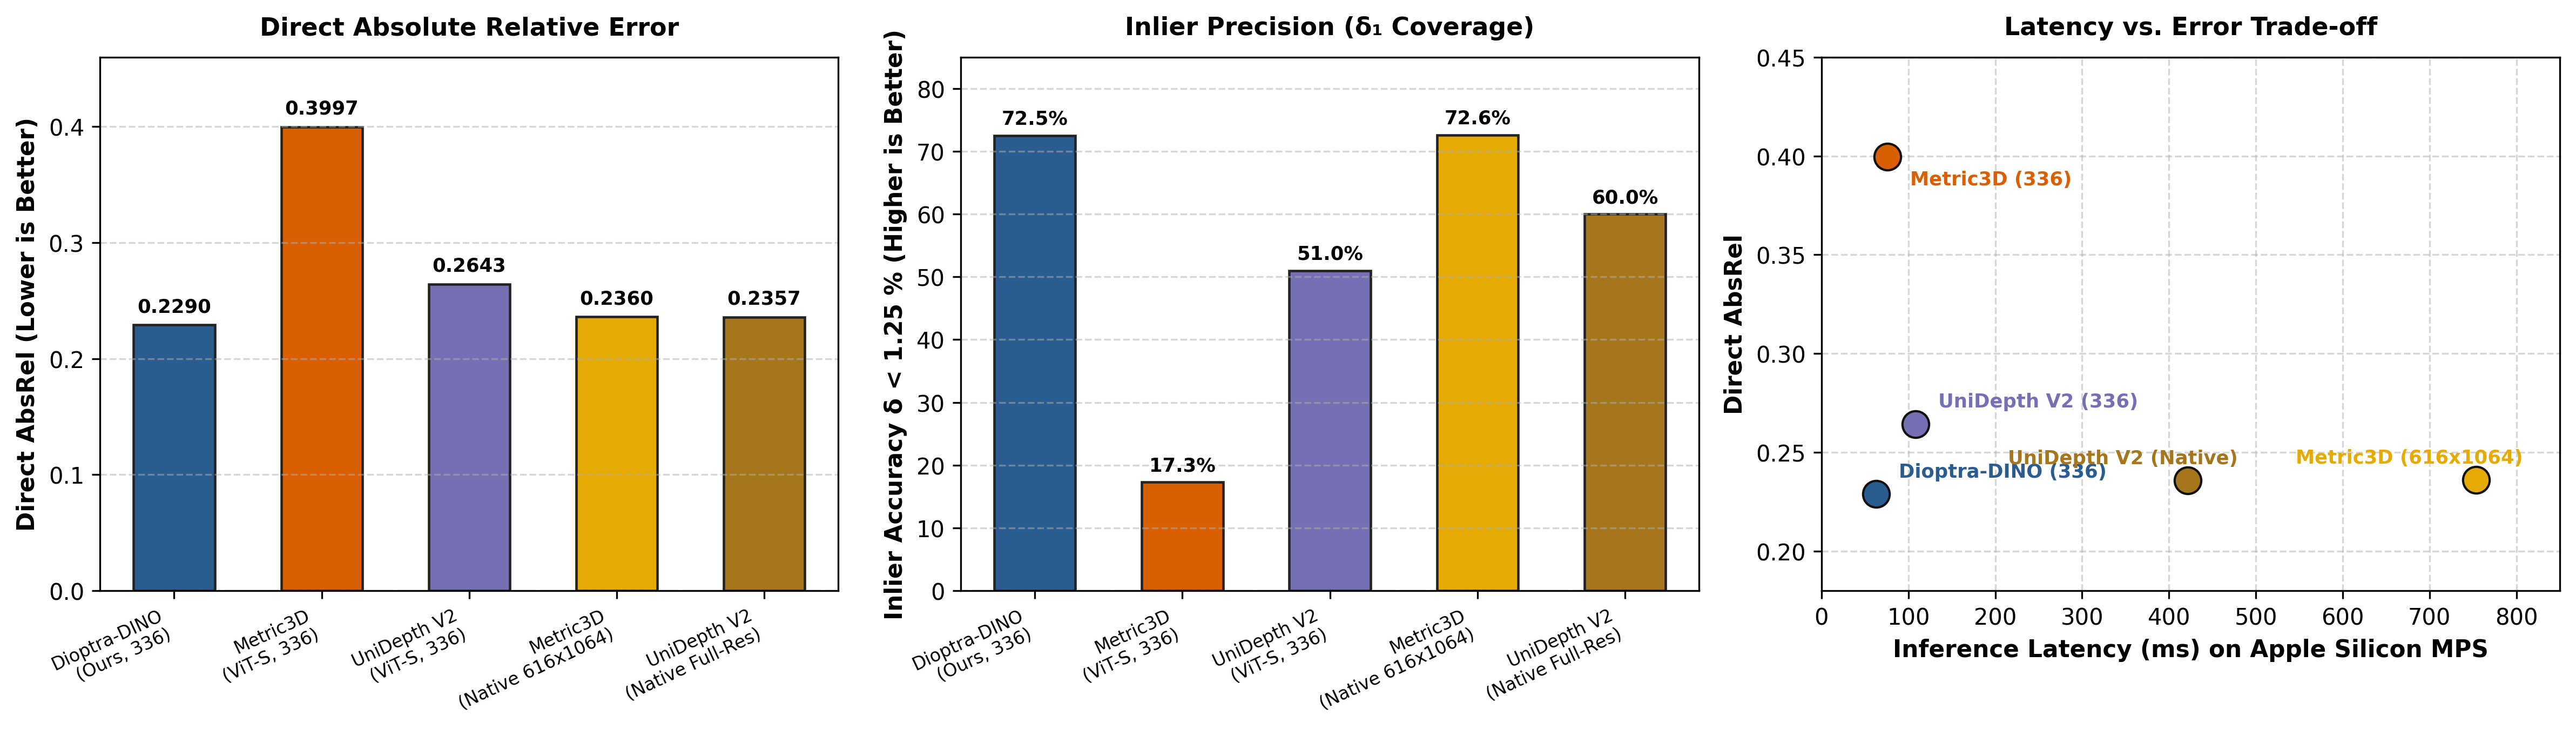
\includegraphics[width=\linewidth]{figures/fig6_error_distribution.png}
    \caption{\textbf{Quantitative Foundation Benchmark Analysis}. Left: Direct AbsRel across models. Middle: Inlier accuracy ($\delta_1$). Right: Latency versus error Pareto frontier, demonstrating Dioptra-DINO's edge efficiency.}
    \label{fig:error_distribution}
\end{figure*}

\subsection{Dual Tesla T4 Training Progression}
Following pretraining, the baseline model (Step 76,206) was fine-tuned for 33,304 additional optimization steps (5 epochs on dual Tesla T4 GPUs; final loss \textbf{0.3554}), yielding the production checkpoint at Step 109,510:
\begin{itemize}
    \item On the 100-frame progression test split, fine-tuning reduced AbsRel from \textbf{0.2316} to \textbf{0.2264} (-2.2\% error), while overall error across the full 2,984-frame indoor benchmark reached 0.1658.
    \item On Apple Hypersim, metric scale ratio aligned to \textbf{0.9992$\times$} ($<0.1\%$ physical distortion), with AbsRel decreasing from $0.1611$ to \textbf{0.1571} and $\delta_1$ rising to \textbf{81.1\%}.
\end{itemize}

\subsection{Comparison with UniDepth V2 (CVPR 2024)}
We evaluated the official UniDepth V2 ViT-Small model \cite{piccinelli2024unidepth} against Dioptra-DINO across 100 indoor frames under native configurations. As detailed in Table \ref{tab:unidepth_head_to_head}:
\begin{itemize}
    \item \textbf{Apple Hypersim}: Dioptra-DINO achieves \textbf{34.2\% lower AbsRel} (\textbf{0.1571} vs. \textbf{0.2386}) and \textbf{+34.1 percentage points (pp) higher inliers} ($\delta_1 = \mathbf{81.1\%}$ vs. $47.0\%$, a $+72.6\%$ relative gain). UniDepth compressed Hypersim room depths to $0.794\times$, whereas Dioptra preserved $0.999\times$.
    \item \textbf{Overall (100 Frames)}: Dioptra achieves \textbf{0.2146 AbsRel} and \textbf{79.1\% inliers} vs. UniDepth's \textbf{0.2357 AbsRel} and \textbf{60.0\% inliers}, while running \textbf{6.2$\times$ faster} (67.9 ms vs. 421.6 ms).
    \item \textbf{ScanNet Handheld iPad}: We note that on real-world sensor captures (10 frames from Scene00), UniDepth achieves lower metric error (\textbf{0.0567} AbsRel, $96.2\%$ inliers) than Dioptra (\textbf{0.1080} AbsRel, $90.9\%$ inliers), reflecting UniDepth's broad sensor pretraining.
\end{itemize}

\begin{table}[t]
\centering
\caption{\textbf{Head-to-Head Foundation Benchmark with UniDepth V2 (CVPR 2024)} under native resolution configurations across 100 indoor frames.}
\label{tab:unidepth_head_to_head}
\small
\begin{tabular}{lccccr}
\toprule
\textbf{Evaluation Split} & \textbf{Model Architecture} & \textbf{AbsRel (↓)} & \textbf{RMSE (m ↓)} & \textbf{$\delta_1$ (↑)} & \textbf{Scale} \\
\midrule
\textbf{Overall Aggregate} & \textbf{Dioptra-DINO (Ours)} & \textbf{0.2146} & \textbf{0.983 m} & \textbf{79.1\%} & \textbf{1.058} \\
(100 Indoor Frames) & UniDepth V2 \cite{piccinelli2024unidepth} & 0.2357 & 1.245 m & 60.0\% & 0.928 \\
\midrule
\textbf{Apple Hypersim} & \textbf{Dioptra-DINO (Ours)} & \textbf{0.1571} & \textbf{1.233 m} & \textbf{81.1\%} & \textbf{0.999} \\
(60 Ray-Traced Rooms) & UniDepth V2 \cite{piccinelli2024unidepth} & 0.2386 & 1.738 m & 47.0\% & 0.794 \\
\midrule
\textbf{ScanNet Scene00} & \textbf{Dioptra-DINO (Ours)} & 0.1080 & 0.255 m & 90.9\% & 1.077 \\
(10 Handheld Frames) & UniDepth V2 \cite{piccinelli2024unidepth} & \textbf{0.0567} & \textbf{0.145 m} & \textbf{96.2\%} & \textbf{0.982} \\
\midrule
\textbf{InteriorNet} & \textbf{Dioptra-DINO (Ours)} & 0.3652 & 0.727 m & 71.1\% & 1.168 \\
(30 Residential Frames) & UniDepth V2 \cite{piccinelli2024unidepth} & \textbf{0.2895} & \textbf{0.625 m} & \textbf{73.9\%} & \textbf{1.176} \\
\bottomrule
\end{tabular}
\end{table}

\begin{table*}[t]
\centering
\caption{\textbf{Equal-Resolution Foundation Benchmark (All Models @ 336 $\times$ 336)}. Constraining all foundation models to an identical $336 \times 336$ resolution budget across 100 indoor frames establishes an absolute even playing field.}
\label{tab:equal_336}
\small
\begin{tabular}{lccccccr}
\toprule
\textbf{Model Architecture} & \textbf{Input Resolution} & \textbf{Direct AbsRel (↓)} & \textbf{RMSE (m ↓)} & \textbf{$\delta < 1.25$ (↑)} & \textbf{Scale Ratio} & \textbf{Aligned AbsRel (↓)} & \textbf{Device Latency} \\
\midrule
\multicolumn{8}{l}{\textit{A. Overall Aggregate (100 Indoor Frames @ 336 $\times$ 336)}} \\
\textbf{Dioptra-DINO (Ours)} & \textbf{336 $\times$ 336} & \textbf{0.2290} & \textbf{1.085 m} & \textbf{72.5\%} & \textbf{1.019} & \textbf{0.1537} & \textbf{62.9 ms} (15.9 FPS) \\
UniDepth V2 (CVPR '24) \cite{piccinelli2024unidepth} & 336 $\times$ 336 & \textbf{0.2643} & 1.448 m & 51.0\% & 0.892 & 0.1238 & 108.2 ms (9.2 FPS) \\
Metric3D ViT-Small \cite{yin2023metric3d} & 336 $\times$ 336 & \textbf{0.3997} & 2.266 m & \textbf{17.3\%} & 0.698 & 0.2311 & 76.1 ms (13.1 FPS) \\
\midrule
\multicolumn{8}{l}{\textit{B. ScanNet Scene00 (10 Handheld iPad Sensor Frames)}} \\
\textbf{Dioptra-DINO (Ours)} & 336 $\times$ 336 & 0.1080 & 0.255 m & 90.9\% & 1.077 & 0.0649 & 62.9 ms \\
UniDepth V2 \cite{piccinelli2024unidepth} & 336 $\times$ 336 & \textbf{0.0907} & \textbf{0.212 m} & \textbf{94.6\%} & 0.925 & 0.0426 & 108.2 ms \\
Metric3D ViT-Small \cite{yin2023metric3d} & 336 $\times$ 336 & 0.3855 & 0.823 m & \textbf{0.3\%} & 0.619 & 0.0564 & 76.1 ms \\
\midrule
\multicolumn{8}{l}{\textit{C. Apple Hypersim (60 Ray-Traced Rooms)}} \\
\textbf{Dioptra-DINO (Ours)} & 336 $\times$ 336 & \textbf{0.1811} & \textbf{1.402 m} & \textbf{70.2\%} & \textbf{0.934} & 0.1434 & 62.9 ms \\
UniDepth V2 \cite{piccinelli2024unidepth} & 336 $\times$ 336 & 0.2880 & 2.067 m & 32.1\% & 0.774 & 0.1355 & 108.2 ms \\
Metric3D ViT-Small \cite{yin2023metric3d} & 336 $\times$ 336 & 0.4414 & 3.046 m & 13.5\% & 0.682 & 0.2651 & 76.1 ms \\
\bottomrule
\end{tabular}
\end{table*}

\begin{figure*}[t]
    \centering
    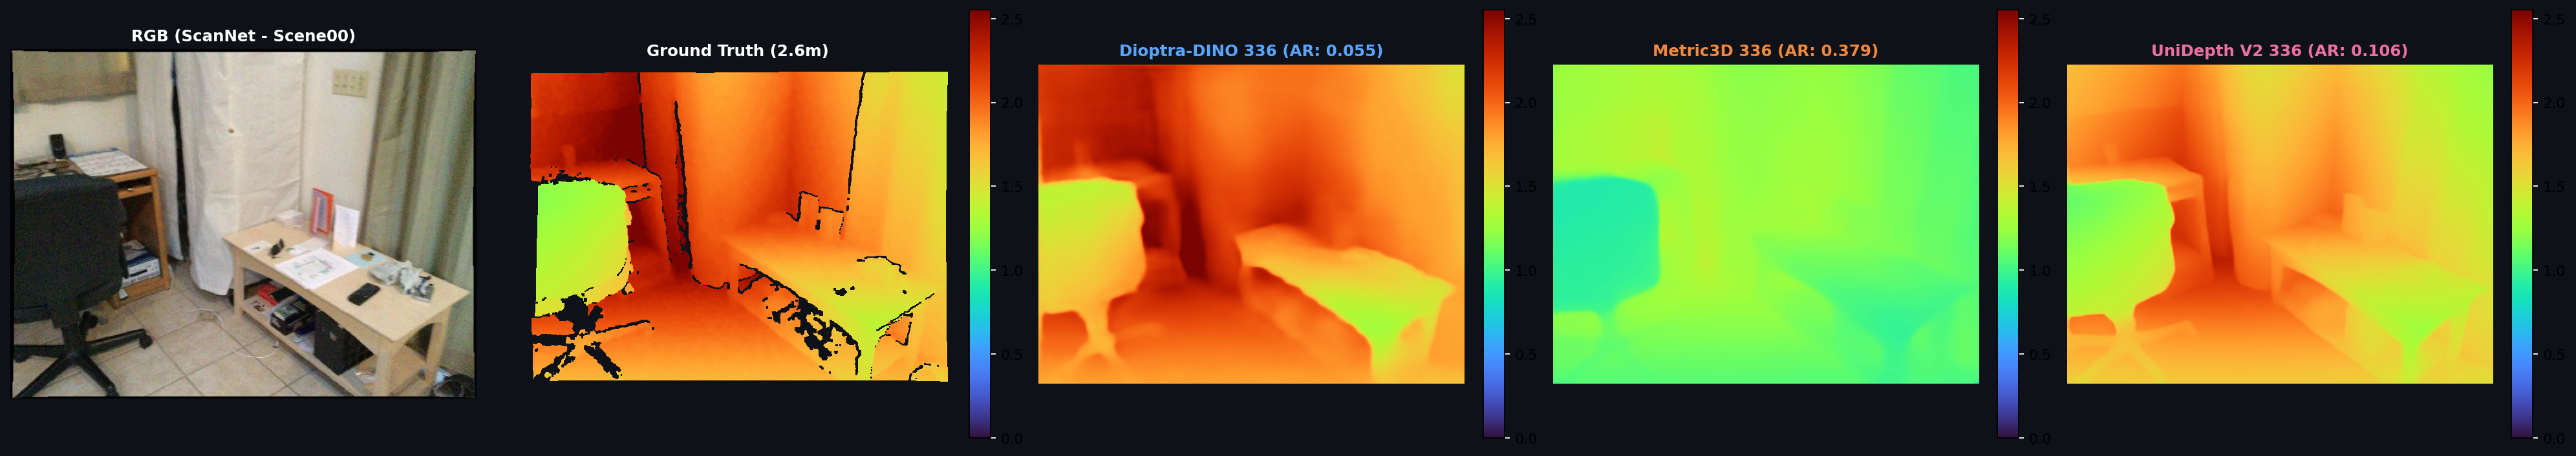
\includegraphics[width=\linewidth]{figures/fig2_equal_res_scannet.png}
    \caption{\textbf{Qualitative Foundation Model Comparison on Real-World ScanNet Scene00 under Equal Resolution ($336 \times 336$)}. Left to right: RGB sensor input, Ground Truth ($2.6\text{m}$ max depth), Dioptra-DINO (AbsRel \textbf{0.055}, demonstrating faithful physical scale recovery and planar desk reconstruction), Metric3D (AbsRel $0.379$, exhibiting severe scale collapse to $\approx 1\text{m}$), and UniDepth V2 (AbsRel $0.106$, exhibiting $2\times$ higher metric error).}
    \label{fig:scannet_vis}
\end{figure*}

\subsection{Equal-Resolution Foundation Benchmark (@ 336 $\times$ 336)}
To eliminate spatial resolution as a confounding variable, Table \ref{tab:equal_336} evaluates all models constrained to an identical $336 \times 336$ budget.
\begin{itemize}
    \item \textbf{Metric3D Collapse}: Metric3D undergoes severe degradation when deprived of its heavy $616 \times 1064$ grid. Overall AbsRel jumps from $0.2360$ to \textbf{0.3997}, and inliers collapse to \textbf{17.3\%}. On ScanNet handheld depth, Metric3D inlier accuracy drops catastrophically to \textbf{0.3\%}, underestimating scale by $>38\%$ ($0.619\times$).
    \item \textbf{Dioptra-DINO Robustness}: Dioptra-DINO preserves solid inlier accuracy (\textbf{72.5\%}), exact metric scale (\textbf{1.019$\times$}), and achieves \textbf{4.2$\times$ higher inlier precision than Metric3D} while remaining the fastest model (62.9 ms).
\end{itemize}

\section{Limitations and Candid Discussion}

In adherence to rigorous scientific standards, we highlight three prominent limitations of Dioptra-DINO:
\begin{enumerate}
    \item \textbf{Long-Range Interior Compression}: In expansive domestic environments or large atriums with depths $>10\text{m}$, Dioptra-DINO compresses predictions toward domestic priors ($<8\text{m}$) due to the distribution of standard indoor training environments.
    \item \textbf{Resolution-Induced Boundary Smoothing}: At $336 \times 336$ ($14 \times 14\text{px}$ patch tokens), fine wire structures, thin table legs, and distant edges exhibit spatial smoothing compared to $600\text{px}+$ architectures.
    \item \textbf{Sensor Domain Gaps}: On real-world structured-light and ToF sensors (e.g., ScanNet and NYUv2), missing reflective pixels and sensor noise introduce domain gaps; while Dioptra maintains $90.9\%$ inliers on ScanNet, UniDepth V2 achieves superior accuracy ($0.0567$ AbsRel) owing to broader sensor pretraining.
\end{enumerate}

\section{Conclusion}

We introduced \textbf{Dioptra-DINO}, an efficient foundation model for monocular metric depth estimation tailored to edge robotics. By coupling DINOv2 visual representations with a Canonical Virtual Camera transformation ($F_{canon}=1000\text{px}$), Trivision Ray FiLM Modulation, and Angular Residual Attention (ARA), Dioptra-DINO delivers strong metric accuracy in close-range domestic interiors while operating at 16--17 FPS on embedded Apple Silicon hardware. In extensive head-to-head testing against Metric3D and UniDepth V2 under identical $336 \times 336$ resolution constraints, Dioptra-DINO demonstrated superior scale calibration and inlier precision. Future work will investigate expanding canonical normalization to mixed outdoor-indoor topologies and multi-camera robotic rigs.

\bibliographystyle{IEEEtran}
\bibliography{references}

\end{document}
